\chapter{Computational details}
\label{sec:Computation}

\section{Settings and dependencies}

The computations were performed on resources provided by Sigma2 - the National Infrastructure for High Performance Computing and Data Storage in Norway, utilizing the Vienna Ab initio Simulation Package (VASP) \cite{vasp1}, \cite{vasp2}, \cite{vasp3}, \cite{vasp4}. As discussed in chapter 5, we employ the projector-augmented-wave method and PBE GGA, in addition to SCAN and HSE06 in certain instances. For the structures studied in this project we found an energy cutoff of 300 eV and 400 eV suitable for electronic and geometric relaxations respectively. In regards to the number of k-points we used a gamma centered mesh with a density of 4 per $\AA^{-1}$. The geometric relaxation of ionic positions and cell volume was carried out in two subsequent runs with convergence criterion of \num{1E-2} $\si{\eV}/\AA$ for the forces and \num{1E-5} eV for the total energy, with Gaussian smearing (ISMEAR = 0 in VASP) and smearing width $\sigma$ equal to 0.05 eV. After successful geometric relaxation the structures underwent a final electronic relaxation with the tetrahedron method with Bl\"{o}ch corrections (TBC, ISMEAR = -5 in VASP), and energy criterion of \num{1E-6} eV between consecutive Kohn-Sham iterations. Calculations with the HSE06 functional in many instances proved difficult to converge electronically. This was solved by two methods: firstly we reduced the density of k-points from 4 $\AA^{-1}$ to 2 per $\AA^{-1}$. Secondly, we found that HSE06 computations converged much quicker with Gaussian smearing compared to the tetrahedron method. Thus, in order to successfully and economically carry out calculations with HSE06 and the tetrahedron method, we first calculated the charge density with Gaussian smearing and reapplied the calculated density in a subsequent HSE06 calculation with the tetrahedron method. Magnetic materials consisting of ferromagnetic elements such as iron, nickel and cobalt, were handled with the setting ISPIN = 2 and the default value of MAGMOM = NIONS * 1.0 in VASP, which specifies the initial magnetic moment for each atom.  Further customization and testing of magnetic orderings such as antiferromagnetic, ferrimagnetic and ferromagnetic were considered beyond the scope of this project.  

The SQS method was implemented through the $\text{generate}-\text{structure}$ script in the Temperature dependent effective potential (TDEP) package, developed by Hellman and Shulumba. Initial cif-files for the relevant structures were obtained from Materials project \cite{Jain2013}. To extract and post-process the VASP calculated data we used VASPKIT \cite{vaspkit} and pymatgen \cite{pymatgen}. 


\section{Material}
In this project we have constructed high-entropy silicides based on the $\beta-$ \ch{FeSi2} compound. The unit cell of this material is in the orthorhombic CMCE space group, and consists of 16 iron atoms and 32 silicon atoms. For each composition we generate five distinct SQSs of equivalent geometry and composition that only vary by atomic configuration. We have emphasized a particular composition of the 3d elements Cr, Fe, Mn, and Ni in a \ch{Cr4Fe4Mn4Ni4Si32} alloy where the 3d elements are distributed equimolarly and occupy the Fe-sites in the $\beta-$ \ch{FeSi2} crystal structure. These SQSs can be seen in figure 6.1. In addition to the \ch{(CrFeMnNi)Si2} composition we have tested alternative compositions with varying distribution and elements generated by an identical procedure consistent with the 48 atom SQS model.

\begin{figure}[H]
\begin{subfigure}{0.5\textwidth}
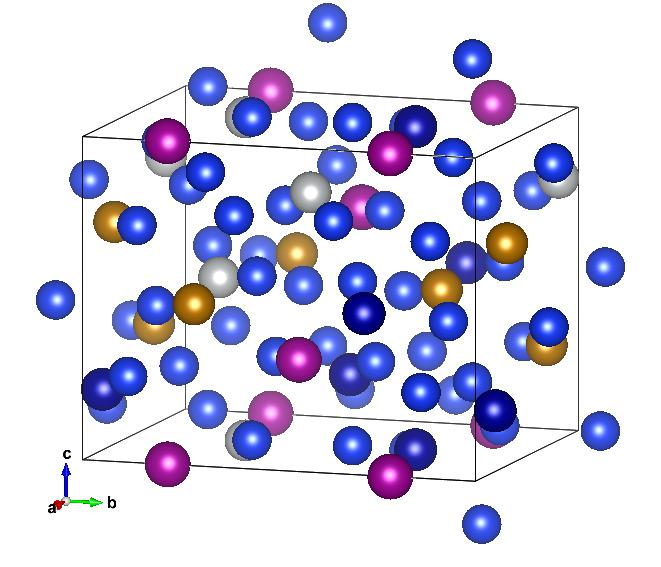
\includegraphics[width=\textwidth]{method/sqs/A.jpg}
\caption{A}
\end{subfigure}
\hfill
\begin{subfigure}{0.5\textwidth}
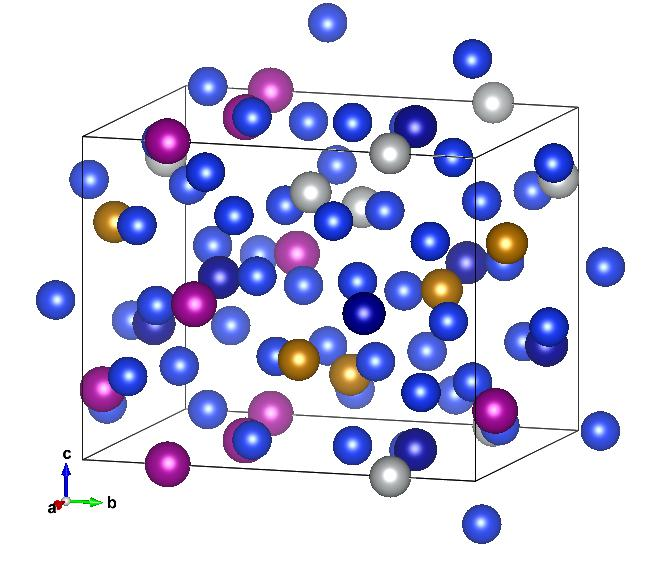
\includegraphics[width=\textwidth]{method/sqs/B.jpg}
\caption{B}
\end{subfigure}
\begin{subfigure}{0.5\textwidth}
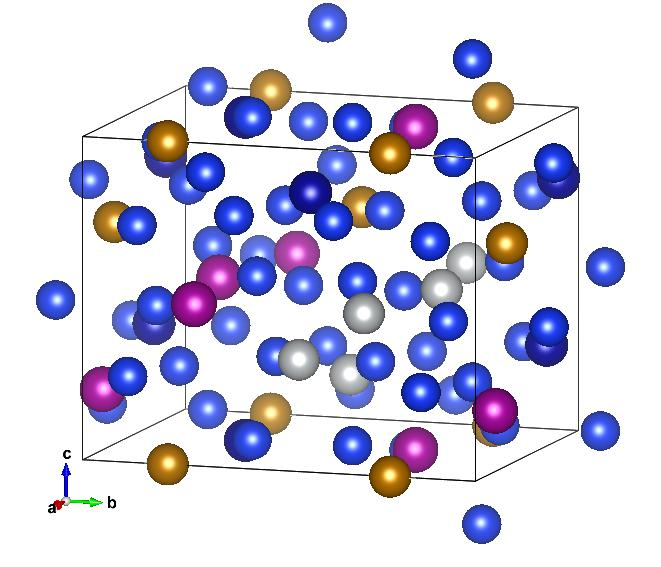
\includegraphics[width=\textwidth]{method/sqs/C.jpg}
\caption{C}
\end{subfigure}
\hfill
\begin{subfigure}{0.5\textwidth}
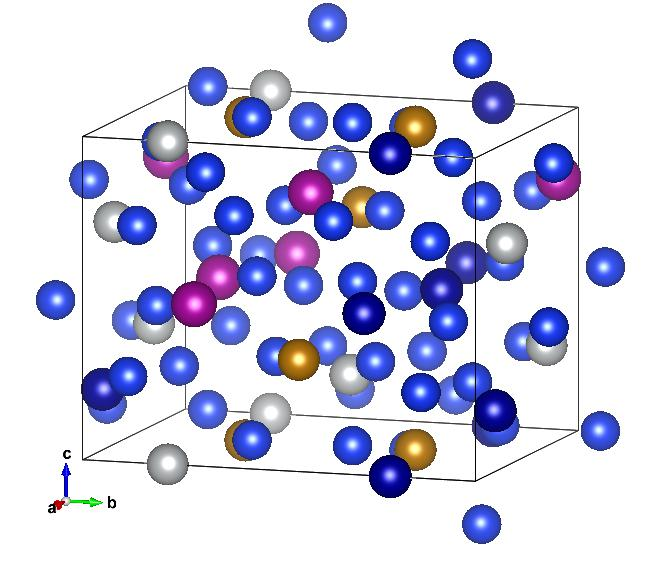
\includegraphics[width=\textwidth]{method/sqs/D.jpg}
\caption{D}
\end{subfigure}
\begin{subfigure}{0.5\textwidth}
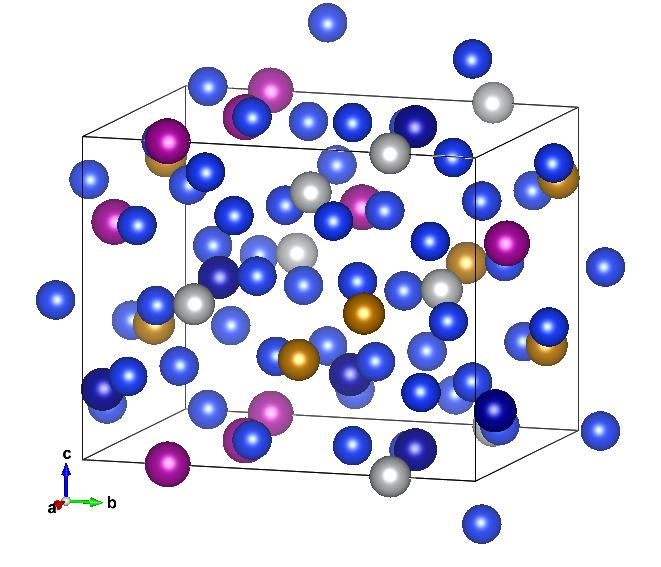
\includegraphics[width=\textwidth]{method/sqs/E.jpg}
\caption{E}
\end{subfigure}
\caption{Five distinct 48-atom SQSs of \ch{Cr4Fe4Mn4Ni4Si32} based on the $\beta-$ \ch{FeSi2} crystal structure. Manganese atoms are represented as purple spheres, chromium as dark blue and silicon as light blue, followed by iron and nickel presented as gold and silver spheres respectively. The respective SQSs are denoted as A, B, C, D and E. Figures illustrated with VESTA \cite{vesta}}
\label{sqs_FeSi2}
\end{figure}